%
% File acl2015.tex
%
% Contact: car@ir.hit.edu.cn, gdzhou@suda.edu.cn
%%
%% Based on the style files for ACL-2014, which were, in turn,
%% Based on the style files for ACL-2013, which were, in turn,
%% Based on the style files for ACL-2012, which were, in turn,
%% based on the style files for ACL-2011, which were, in turn, 
%% based on the style files for ACL-2010, which were, in turn, 
%% based on the style files for ACL-IJCNLP-2009, which were, in turn,
%% based on the style files for EACL-2009 and IJCNLP-2008...

%% Based on the style files for EACL 2006 by 
%%e.agirre@ehu.es or Sergi.Balari@uab.es
%% and that of ACL 08 by Joakim Nivre and Noah Smith

\documentclass[11pt]{article}
\usepackage{acl2015}
\usepackage{times}
\usepackage{url}
\usepackage{latexsym}
\usepackage{graphicx}
\usepackage{booktabs}
\usepackage{multirow}

%\setlength\titlebox{5cm}

% You can expand the titlebox if you need extra space
% to show all the authors. Please do not make the titlebox
% smaller than 5cm (the original size); we will check this
% in the camera-ready version and ask you to change it back.


\title{LSTM Recurrent Network for Step Counting based on WeAllWork Dataset}

\author{Ziyi Chen \\
  Computer Science  \\
  Unversity of California Santa Cruz\\
  {\tt zchen139@ucsc.edu}}
  
  

\date{}

\begin{document}
\maketitle
\begin{abstract}

Smartphone offers various sensors such as accelerometers and gyroscope that can be used for pedometer and environment-related events. This paper trains an LSTM recurrent network for counting the number of steps taken by both blind and sighted users, based on WeAllWork Dataset. The model is built separately for blind volunteers using long canes and guided dog as well as sighted volunteer for the Leave-One-Out training modality.

\end{abstract}

\section{Introduction}

Originally used by sports and physical activity tracking, pedometers are now becoming popular as daily exercise counter and motivator. Pedometers count each step a person takes by detecting the motion of the person's hands or hips. Step counters are being integrated into an increasing number of portable consumer electronic devices such as music players, smartphones, and mobile phones. 

With the increasing ubiquity of smartphones, users are now carrying around a plenty of sensors like accelerometers, gyroscope, magnetometer with them wherever they go. There are various of step counting apps in smartphones. Step counters can also be used for estimating the distance and the position in indoor pedestrian navigation systems, which is especially helpful not only for blind people, but also for sighted people who need directional information in unfamiliar places.

This paper proposes an LSTM model trained by indoor walking sensor data of iPhone and annotated data of cpro from WeallWalk dataset as training data and label, to predict left or right steps and calculate the count of steps. The cpro is attached to the shoes so it can provide precise times of heel strike. In the dataset, blind volunteers using long canes and guided dogs as well as sighted volunteers have different features of gaits, so we separately build the model and calculate the error rate of three metrics. In practice, pedometers don't have any annotated data from a new user, so we apply leave one person out pedometers to test the accuracy of our model. Three error metrics splitting intervals differently estimate the overcount and undercount of steps. We also try different parameters for the LSTM models such as timesteps and training steps to compare the difference of output.



\section{Background and Related Work}

\subsection{Step Counting}

\begin{figure*}[ht]
\centering
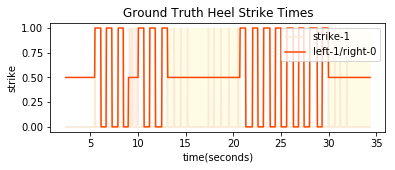
\includegraphics[scale=0.5]{ground_truth_2}
\caption{Example heel strike times of T1\_ID1\_WC.xml from 2.4s to 34.4s. The first step is left feet at 5.4761s. A feature motion (the participant walked into the wall, stopped, and moved to the left) happened from 9.041862s to 10.041862s. Two turn motion, Turn east to south from 13.1752s to 20.7419 and Turn south to east from 30.0419 happened. All data before first step as well as feature and turn data are removed.}
\label{fig:ground_truth}
\end{figure*}


Automatic step counting has received substantial attention from both research and commercial. There is a wealth of studies on the use of inertial sensors for detecting and characterizing walk-related activities. Pedometers are usually portable and electronic or electromechanical. It can be embedded in shoes, in a smartwatch, in a smartphone, and attached to one’s ankles or hung on the belt.

\cite{tomlein2012advanced} introduces step detection and intelligent detection of cheating based on smartphone sensors.
\cite{naqvib2012step} presents a method for counting the number of steps taken by a user, while walking at any variable speed, using the smartphone-based accelerometer.

\cite{brajdic2013walk} evaluates common walk detection (WD) and step counting (SC) algorithms applied to smartphone sensor data. The results favor the use of standard deviation thresholding (WD) and windowed peak detection (SC) with error rates of less than 3\%.
A variety of algorithms have been proposed for stride event detection from inertial sensor time series. Some of these algorithms operate on the accelerometer data, while others use data from the gyros. For example, The Window Peak Detection algorithm (WPD) runs a moving average window on the smoothed accelerometer magnitude to find peaks associated with a heel strike. \cite{alzantot2012uptime} UPTIME (Ubiquitous Pedestrian Tracking usIng Mobile phonEs) uses the de-trended magnitude of acceleration in a finite state machine (FSM), with six states to identify the peaks associated with heel strikes. \cite{mannini2011hidden} HMM-acc trains a Hidden Markov Model (HMM) to discern the different phases during a gait period. 
%\cite{jayalath2013gyroscope} ZC-gyro searches for zero crossings (ZC) within a moving window of the data from the gyro aligned with the medial-lateral axis. 


Recent approaches to step detection include the use of recurrent neural networks. Researchers use RNN for evaluating and optimising accelerometer-based gesture recognition, self-calibration, pedestrian dead reckoning.
\cite{edel2015advanced} uses Bidirectional Long Short-Term Memory Recurrent Neural Networks (BLSTM-RNNs) for step detection, step length approximation as well as heading estimation.

Whereas the vast majority of step counting algorithms have been developed for able-bodied ambulators, some researchers have addressed the performances of these algorithms with sensors carried by people with some level of mobility impairment such as \cite{haegele2015validation} and \cite{holbrook2011validation}. 



\subsection{WeAllWalk Dataset}

WeAllWalk dataset \cite{flores2016weallwalk} contains inertial sensor time series collected from ten blind walkers using a long cane or a guide dog and five sighted walkers. The participants walked through fairly long and complex indoor routes that included obstacles to be avoided and doors to be opened. Inertial data was recorded by iPhone 6s carried by participants in their pockets. Ground truth heel strike times were measured by two small inertial sensor units attached to the participants’ shoes. The data set contains a mobility impairment that may result in a gait pattern that is quite different than for sighted walkers. The data is subdivided into straight paths and turns and carefully annotated, with special events (or features, such as bumping into an obstacle) individually identified and marked. Based on the data in WeAllWalk, they conducted two parallel analyses of algorithms for step counting and turn detection from inertial sensor data. Step counting is a widely used technique for approximate odometry; in combination with turn detection, it provides a simple localization strategy for walkers inside a building. 


\section{Implementation}
We propose an LSTM model trained by indoor walking sensor data of iPhone to predict left or right steps for step counting. Since Blind volunteers using long canes and guided dogs as well as sighted volunteers have different features of gaits, we separately build the model and calculate the error rate of three metrics. Also, we only considered straight segments in the paths, since the gait is more likely to be regular rather than turn segments, and avoided segments labeled as features such as a door need to be opened and an obstacle needs to be eluded. We try different parameters for the LSTM model and add a dropout layer to make the result more robust.

\subsection{Data Preprocess}

\begin{figure*}[ht]
\centering
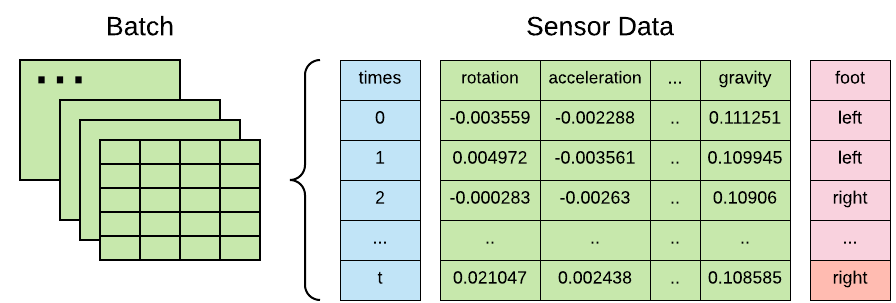
\includegraphics[scale=1]{input2}
\caption{Input (green) and output (pink) example for LSTM. Use previous timesteps(t) records of sensor data (green blocks) to predict the last foot step (last pink foot). The fisrt timesteps(eg. t=50) outputs of each segement are determined by intermediate outputs (light pink) since they don't have enough previous record. Shuffle and divide train data into the small batchs as inputs.}
\label{fig:batch_sensor_data}
\end{figure*}

WeAllWalk dataset contains detailed maps of indoor paths, scripts to facilitate visualization of all the information in this data set and recorded sensor data for all users and all paths.

We use two kinds of file from the dataset. First is the CSV file of iPhone sensor data as input. It contains records of all iPhone sensors. There are total 39 columns of sensor data and some of them are more useful such as rotation rate and user acceleration.

Second is the XML files that contain annotated ground truth data for all the paths walked by all the participants as labels. Each file contains start and end times for each segment the user walked through and feature information like the left or right foot as well as direction. We only train and test the step detection algorithms on data acquired while traversing straight segments in the paths, where gait is assumed to be regular, and avoided segments labeled as features. This is because the notion of “step” is not well defined in such situations. In general, we argue that step counting only really matters during regular ambulation, as an indirect way to measure distances traversed.

Since the XML files only contain heel strike times, we cannot use it as labels directly. It is unreasonable to predict next strikes times by previous records. If we regard heel strike times as 1 and other times as 0, then the labels are unbalanced. So we apply the same sampling rate as CSV files and transform the XML file to 0-1 in which left steps as 1 and right steps as 0 to make the data balanced.

As shown in picture \ref{fig:ground_truth}, the light color line of strike time is the original data from XML file. It is transformed to redline which regards left as 1 and right as 0. We also remove the turn data(light yellow background part) and feature data(light red background part). Then we windowed the data by timesteps size for corresponding sensor data and labels.

\begin{figure*}[ht]
\centering
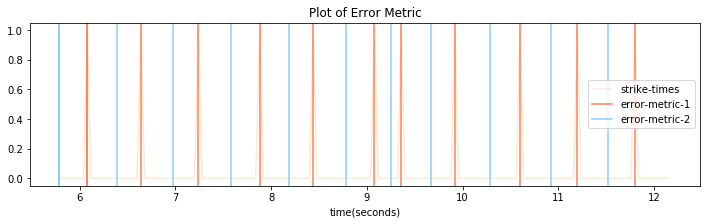
\includegraphics[scale=0.6]{error_metric}
\caption{Example of three error metrics. Assume above plot is a entire segement. Error metric 1 (read line) split intervals exactly at each heel strike times. Error metric 2 (blue line) split intervals exactly at middle of every two continues heel strike times. Error metric 3 calculate undercount and overcount for the entire segment.}
\label{fig:error_metric}
\end{figure*}



\subsection{LSTM Model}
Long short-term memory (LSTM) network is a recurrent neural network. It can be used as blocks of recurrent neural network(RNN) network. There are different types of LSTMs, which differ in the components or connections that they have. An LSTM layer consists of a number of recurrently connected memory blocks. Each block contains one or more recurrently connected memory cells and three multiplicative units, the input, output, and forget gates, which control the information flow inside the memory block. The surrounding network can only interact with the memory cells via the gates. In other words, these gates and the memory cell allow an LSTM unit to adaptively forget, memorize and expose the memory content. Due to above characteristic, LSTM is suitable to predict time series such as step counting.

We use TensorFlow to implement LSTM network. TensorFlow is an open-source software library that can be used for machine learning applications such as neural networks. It supports both CPU and GPU that can be imported as a python library. TensorFlow uses a data flow graph to represent computation in terms of the dependencies between individual operations. We first define the data flow graph and then create a session to run the graph. The Saver class of TensorFlow can easily add ops to save and restore variables to and from checkpoints, which map variable names to tensor values.

As shown in picture \ref{fig:LSTM}, a two-layer RNN network with basic LSTM cell and dropout wrapper are built for training with squared difference loss function. The input is a list of metrics with the row of timesteps and col of sensor data. For Example, we want to use previous timesteps ($=50$) record of sensor data to predict the result, each sensor data contains input number ($=6$) values of rotation rate and user acceleration. So the matrix size is timesteps multiply input number($50 \times 6$). All such metrics form the input list and is transformed to tensor. Since the dataset is big and there are more than one hundred thousand elements in input list which would make the training process very slow, we shuffle and divide train data into the small batch (batch size = 256) and feed the batch to model.

\begin{figure}[ht]
\centering
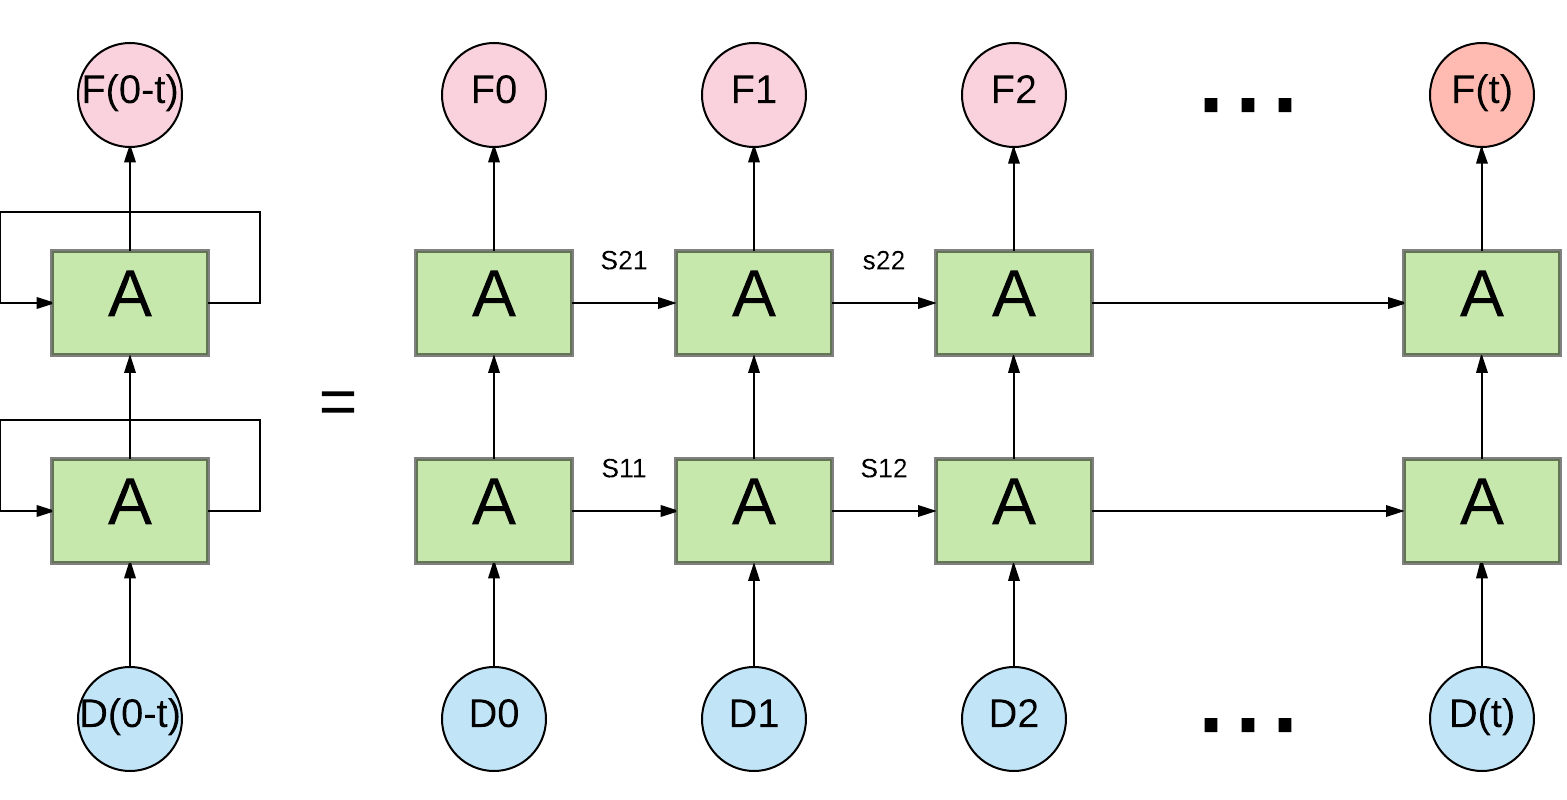
\includegraphics[scale=0.3]{LSTM3}
\caption{Two layer LSTM recurrent network. Each green block is a LSTM Block with number of hidden nodes. Blue circle D represent for sensor data, s is the lstm state, pink circle F is the output feet, which is a float value around 0 to 1.}
\label{fig:LSTM}
\end{figure}


There are two ways of output. One is to use previous timesteps data to predict only the last step result, which is a float value around 0 to 1. We use 0.5 as the border to classify left and right steps. And the heel strike times is when 0 change to 1 or 1 change to 0. The other is to use previous timesteps data to predict corresponding timesteps step results. The first one cannot predict the first timesteps result, but it is more precise since all result is predicted by previous timesteps record. Most outputs that have enough previous records use first way to calculate.


\begin{figure*}[ht]
\centering
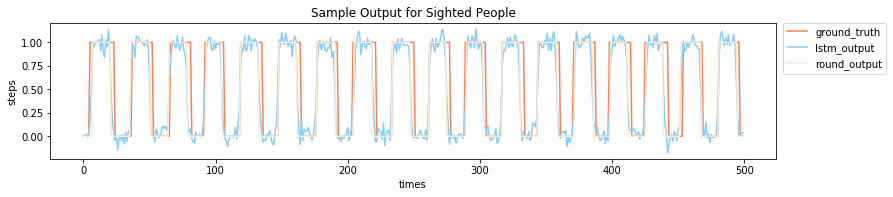
\includegraphics[scale=0.5]{output_sighted}
\caption{Sample output for sighted people. The float output (blue line) is swing around 0 or 1. The predicted round ouput (yellow line) is quite similar to the ground truth data (red line).}
\label{fig:output_sighted}
\end{figure*}



\subsection{Error Metrics}
The round of result is a list of left/right step corresponding to origin step. Then calculate the accuracy rate of the result, which is the proportion of correct numbers (left is predicted to be left and right is predicted to be right) and total numbers.


The quality of the step counting model was measured using three different metrics. The first metric looks at the number of steps detected within each time interval $[T_i, T_{i+1}]$ separating two consecutive ground-truth heel strikes. Ideally, exactly one step should be detected within one interval $[T_i, T_{i+1}]$. If no steps are detected in $[T_i, T_{i+1}]$, then an undercount event is recorded. If steps are detected within that interval, the overcount events are recorded. The cumulative number of undercount and overcount events are computed and normalized (divided) by the number of ground-truth steps.

The second metric is similar to the first,  but it looks at the number of steps detected within each time interval $[\frac{T_{i-1}+T_i}{2}, \frac{T_i+T_{i+1}}{2}]$ separating two consecutive ground-truth heel strikes. Ideally, exactly one step should be detected within one interval $[\frac{T_{i-1}+T_i}{2}, \frac{T_i+T_{i+1}}{2}]$. The undercount and overcount is calculated same as first metric. The metric can decrease error when one step is detected sightly earlier ($t_i<T_i$) and the next step is detected sighted later ($t_{i+1}<T_{i+1}$). For this case, interval $[T_i, T_{i+1}]$ has one undercount, and interval $[T_{i-1}, T_i]$ and $[T_{i+1}, T_{i+2}]$ have one overcount.

The third metric simply computes the difference between the number of detected steps within each segment and the number of ground-truth steps within the same segment. The difference between the two is recorded as an undercount value if negative, as an overcount if positive. Undercount and overcount values are then summed together over all segments, and normalized by the total number of ground-truth steps.

Note that the normalized undercount and overcount values obtained by the error metric 1 and 2 metrics is always larger than or equal to the corresponding values computed by the metric 3, as missed counts or double counts between a time interval $[T_i, T_{i+1}]$ may even out over multiple steps. While the more lenient metric 5 may be appropriate when measuring step counts over long hauls, the more conservative metric 1 may be useful when fine-grained tracking is desired. When training and benchmarking the algorithms, the sum of overcount and undercount rates is used for both error metrics.

\begin{figure*}[ht]
\centering
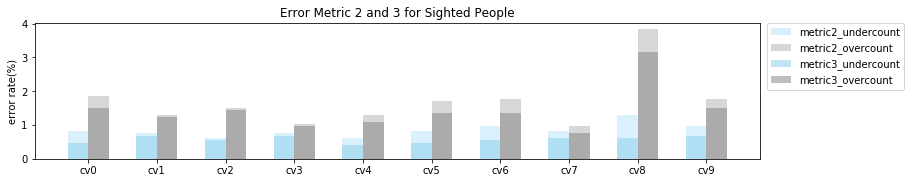
\includegraphics[scale=0.5]{error_metric_23_na_10fold}
\caption{Error metric 2 and 3 for 10 fold cross validation of sighted people.The error rate of metric 2 is always higher than metric 3. The undercount error (blue blocks) is less than overcount error (grey blocks). Detailed values is shown in table. Fold 3 and 4 have better result and fold 8 has a relatively bad result.}
\label{fig:error_metric_23_na_10fold}
\end{figure*}

\begin{figure*}[ht]
\centering
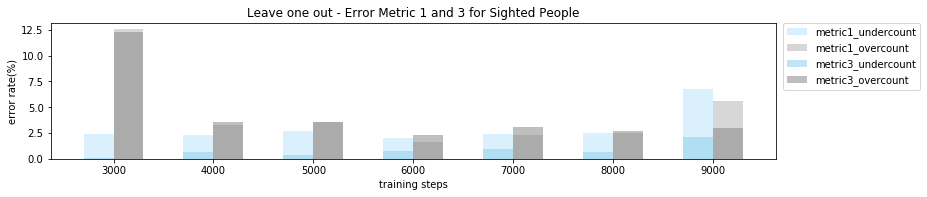
\includegraphics[scale=0.5]{error_metric_13_na_step}
\caption{Error metric 1 and 3 for leave one out of sighted people with regrad to training steps. The error rate of metric 1 is always higher than metric 3.}
\label{fig:error_metric_13_na_step}
\end{figure*}


\section{Experience}

We preprocessed the WeAllWalk data to train LSTM model for the different communities represented in the dataset. 
We experience two ways of splitting train and test data. First is simply mixed all data, and both train and test data contain records for every participant and for every segment. Second is leave one person out, which means train and test data wouldn't contain the same person. Because in practical use, we don't have the annotated data from new users. 
Figure x-x show the error for metric 1, 2 and 3 for each community for mixed data under the Stratified Leave-One-Out training modality.

The model is trained with different input numbers, timesteps, output number, hidden layer number, optimizer, learning rate and training steps. We first try different optimizers with various learning rate and find that AdamOptimizer with learning rate around 0.001 can make it convergence, and then fix the two parameters. 
Increasing timesteps would make input larger and slow the training step for every step, while less training steps are needed to convergence, so overall time is similar. Also when timesteps are larger, it is easier to overfit.

\subsection{Sighted people}
There are total 12w+ input data of sighted people, we split it into 10w+ train data and 2.5w+ test data. Each input data is a 3-dimensional tensor, with a shape of batch size $\times$ timesteps $\times$ number of sensor data.

For mixed train and test data, we apply 10 folds cross-validation. A good sample result is shown in picture \ref{fig:output_sighted}. The float value of output swings around 0 or 1. So it is reasonable to use 0.5 to classify left or right step ($>0.5$ is left step, $<=0.5$ is right step). The round result is similar to the ground truth data. However, not all result is as good as this sample. Some result has a certain offset between ground truth data and predicted output, some result function shakes more fiercely and not all values are close to 0 and 1. Thus there tend to be more strikes if the output value shakes around 0.5. So the overcount rate is always higher than the overcount rate.

\begin{figure}[ht]
\centering
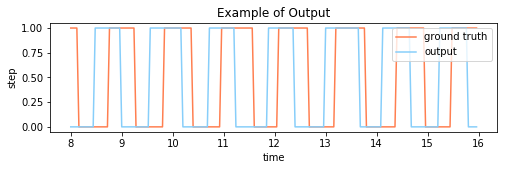
\includegraphics[scale=0.4]{output_ex_offset}
\caption{Sample output of offset. In this case, error metric 1 works better than error metric 2.}
\label{fig:output_ex_offset}
\end{figure}


Since there are 6 error values, it difficult to determine a weighted format over each error rate and tell which model is better. So all ten result is shown in picture \ref{fig:error_metric_23_na_10fold}. The result doesn't have much difference from each other. The undercount rate is around 1\% and the overcount rate is less than twice of undercount rate (2\%). The value of error rate is shown in table \ref{label_metric23_sighted}. The error rate is much higher than error rate for metric 2 and 3, the undercount rate is similar top overcount rate (around 20\%) as shown in picture \ref{fig:error_metric_1_na_10fold}. The reason that caused such situation is described in picture \ref{fig:output_small_metric2}. So the error rate of undercount and overcount is similar since when a undercount happened it is likely to cause a overcount.

\begin{figure}[ht]
\centering
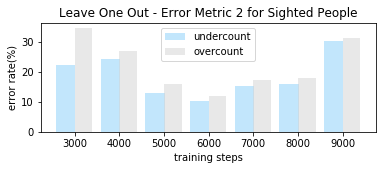
\includegraphics[scale=0.55]{error_metric_2_na_step}
\caption{Error metric 1 and 3 for 10 fold cross validation of sighted people.The error rate of metric 1 is always higher than metric 3 with regrad to training steps.}
\label{fig:error_metric_2_na_step}
\end{figure}


\begin{figure*}[ht]
\centering
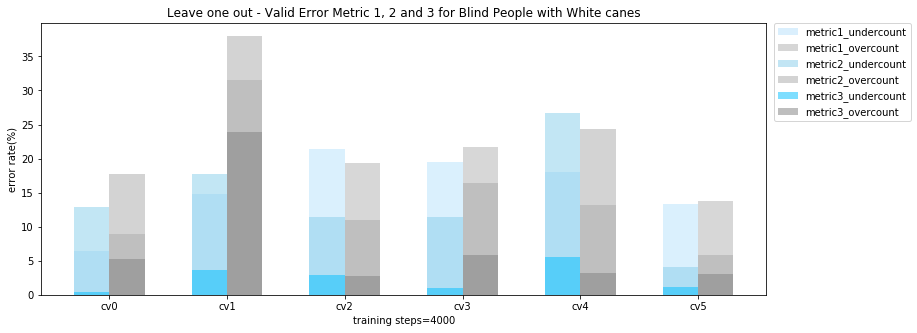
\includegraphics[scale=0.5]{error_metric_wc_10fold_valid4000}
\caption{Leave one out - Valid Error for Blind People with White Canes}
\label{fig:error_metric_wc_10fold_valid4000}
\end{figure*}


\begin{figure*}[ht]
\centering
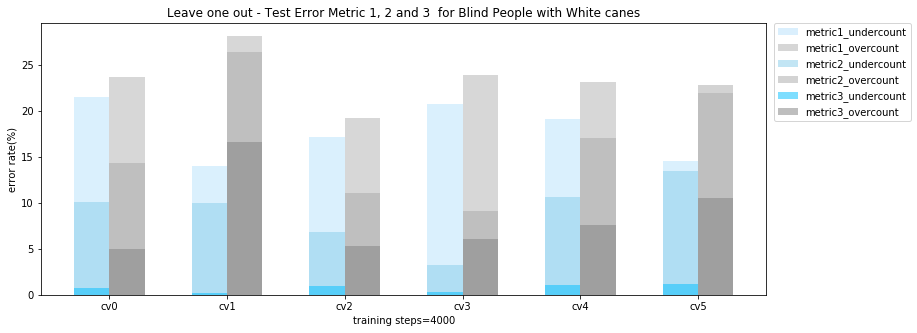
\includegraphics[scale=0.5]{error_metric_wc_10fold_test4000}
\caption{Leave one out - Test Error for Blind People with White Canes}
\label{fig:error_metric_wc_10fold_test4000}
\end{figure*}

For leave one person out method, the result is shown in picture \ref{fig:error_metric_2_na_step}. The best result is got after around 6000 steps. When the training step is less than 4000, the function is underfitted, while the training steps are larger than 7000, the function is overfitted. In this case, metric 2 has bad performance as shown in picture \ref{fig:error_metric_2_na_step}. This is because there is an offset around half of each interval as shown in the picture. The offset is good for metric 1 but bad for metric 2. The result for error metric 1 and 3 is shown in \ref{fig:error_metric_13_na_step}. The error rate for step=600 is 2.5\%, and metric 2 undercount rate is 1\%.

When the train and test data both contains the sensor data from certain people, then the prediction of left or right feet is quite accurate, so the error (metric 2 and 3) of step counting is small. However, if the sensor data of train and test are from different people, then there would be a certain offset for test data, and the accuracy of left and right foot is low. But the error (metric 1 and 3) is still small since the offset is similar for each heel strikes as shown in picture \ref{fig:output_ex_offset}. It may because different people have different gaits.

\subsection{Blind People with White Canes}
A white cane is used by many people who are blind or visually impaired. Primarily it aids its user to scan their surroundings for obstacles or orientation marks, but is also helpful for other traffic participants in identifying the user as blind or visually impaired and taking appropriate care.

There are total 20w+ input data of blind people with white canes, participants 1, 2, 3, 5, 6, 7, 8 have sensor data for six paths. So use participant 8 as test data, and remain 6 people data for 6 fold cross validation for leave one out. The valid and test result is shown in picture \ref{fig:error_metric_wc_10fold_valid4000} and \ref{fig:error_metric_wc_10fold_test4000} with training step=4000. The result is worse than mix data. There is no clear relationship between the correctness of valid data and test data. The training data contains six different people, which is not a big number. If we have annotated data from more people, LSTM model may detect common features of blind people and provide a better result.

\begin{figure*}[ht]
\centering
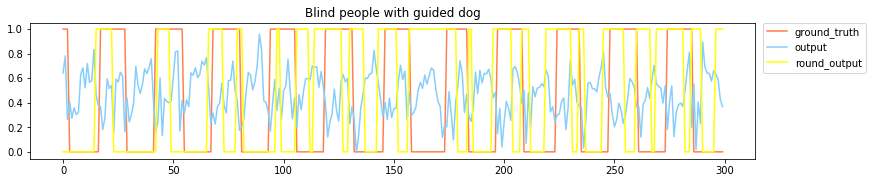
\includegraphics[scale=0.5]{blind_gd}
\caption{Sample output of blind people with guided dog.}
\label{fig:blind_gd}
\end{figure*}


\subsection{Blind People with Guide Dogs}

The guide dog is assistance dogs trained to lead blind and visually impaired people around obstacles. The human does the directing, based on skills acquired through previous mobility training. The handler might be likened to an aircraft's navigator, who must know how to get from one place to another, and the dog is the pilot, who gets them there safely.

There are only 3 people walked with the guided dog, each has 3w+ data. So we regard one people as train data, one as valid data, and the other as test data. The result is bad as shown in \ref{fig:blind_gd}. Although mixed data shows good performance around 5\% for metric 2 and 2\% for metric 3, it is not likely to predict the strike heel times of a person from only one different person.

\begin{table}[]
\centering
\caption{Error of blind people with guided dog}
\label{my-label}
\begin{tabular}{llll}
\hline
error(\%)                &            & valid & test  \\ \hline
metric1                  & undercount & 23.90 & 10.18 \\
                         & overcount  & 26.14 & 25.75 \\ \hline
\multirow{2}{*}{metric2} & undercount & 22.56 & 12.27 \\
                         & overcount  & 29.03 & 19.49 \\ \hline
\multirow{2}{*}{metric3} & undercount & 4.52  & 0.53  \\
                         & overcount  & 10.98 & 17.75 \\ \hline
\end{tabular}
\end{table}


\section{Conclusion and Future Work}

We train an LSTM model trained by indoor walking sensor data of iPhone and annotated data of cpro from WeallWalk dataset as training data and label, to predict left or right steps and calculate the count of steps. The cpro is attached to the shoes so it can provide precise times of heel strike. In the dataset, blind volunteers using long canes and guided dogs as well as sighted volunteers have different features of gaits, so we separately build the model and calculate the error rate of three metrics. In practice, pedometers don't have any annotated data from a new user, so we apply leave one person out pedometers to test the accuracy of our model. There are three error metrics splitting intervals differently to estimate the overcount and undercount of steps. We also try different parameters for the LSTM models such as timesteps and training steps to compare the difference of output. As shown in picture \ref{fig:overcount} and picture \ref{fig:undercount}, simple classify left and right step by 0.5 may cause the overcount or undercount. So we can use a better way to distinguish left step from the right step. In this paper, we only use the data of straight segments, avoiding turn segment and other features. We could consider about turn data and feature motions. We now only use rotation rate and user acceleration as input, we can also try more sensor data in future.

\begin{figure}[ht]
\centering
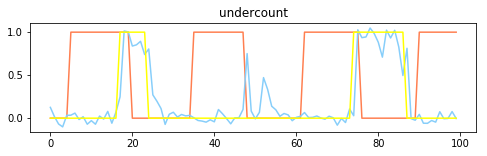
\includegraphics[scale=0.4]{undercount}
\caption{Sample of undercount.}
\label{fig:undercount}
\end{figure}

\begin{figure}[ht]
\centering
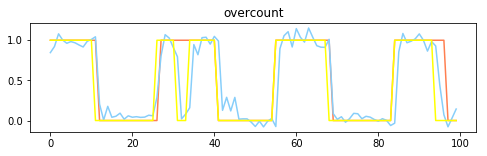
\includegraphics[scale=0.4]{overcount}
\caption{Sample of overcount.}
\label{fig:overcount}
\end{figure}


\begin{figure*}[ht]
\centering
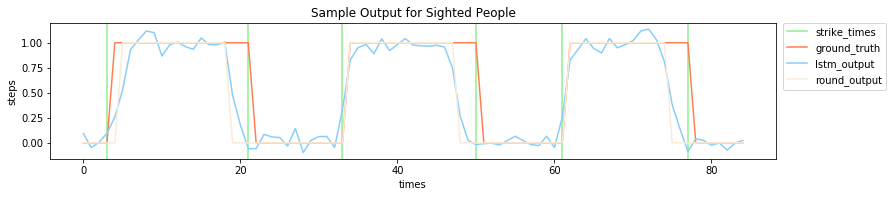
\includegraphics[scale=0.5]{output_small_metric2}
\caption{Bad sample for error metric 1. The green line is the split line for the interval of error metric 1. There are random offset between actual strikes times and predicted strike times. In this case, first, third and fifth interval has one overcount, second and fourth interval has one undercount}
\label{fig:output_small_metric2}
\end{figure*}




\begin{figure*}[ht]
\centering
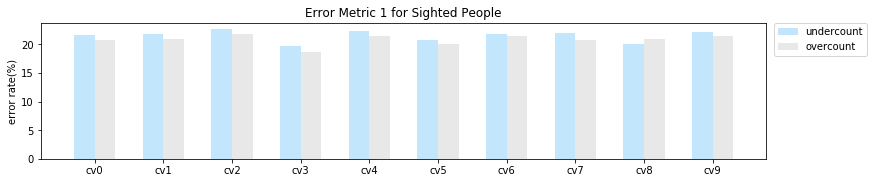
\includegraphics[scale=0.5]{error_metric_1_na_10fold}
\caption{Error metric 1 for 10 fold cross validation for sighted people. The error rate is much higher than error rate for metric 2 and 3 as shown in picture. The reason that caused such situation is described in picture.}
\label{fig:error_metric_1_na_10fold}
\end{figure*}


\begin{figure*}[ht]
\centering
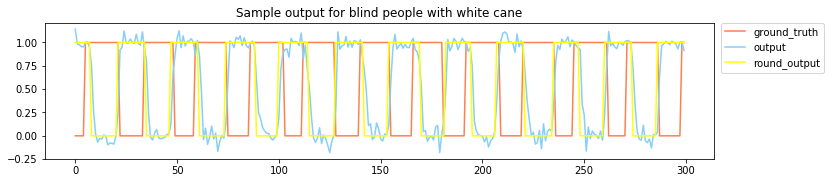
\includegraphics[scale=0.5]{output_wc_1}
\caption{Sample output of blind people with white cane.}
\label{fig:output_wc_1}
\end{figure*}

\begin{figure*}[ht]
\centering
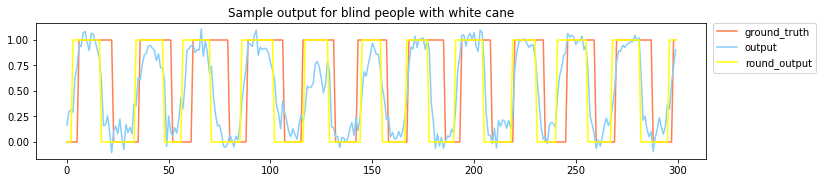
\includegraphics[scale=0.5]{output_wc_2}
\caption{Sample output of blind people with white cane.}
\label{fig:output_wc_2}
\end{figure*}




\begin{table*}[]
\centering
\caption{Error metric 2 and 3 for 10 fold cross validation of sighted people}
\label{label_metric23_sighted}
\begin{tabular}{llllllllllll}
\hline
error(\%)                &            & cv0   & cv1   & cv2   & cv3   & cv4   & cv5   & cv6   & cv7   & cv8   & cv9  \\ \hline
metric1                  & undercount & 0.82  & 0.75  & 0.62  & 0.75  & 0.62  & 0.82  & 0.96  & 0.82  & 1.3   & 0.96 \\
                         & overcount  & 1.85  & 1.3   & 1.5   & 1.03  & 1.3   & 1.71  & 1.78  & 0.96  & 3.83  & 1.78 \\ \hline
\multirow{2}{*}{metric2} & undercount & 0.48  & 0.68  & 0.55  & 0.68  & 0.41  & 0.48  & 0.55  & 0.62  & 0.62  & 0.68 \\
                         & overcount  & 1.5   & 1.23  & 1.44  & 0.96  & 1.09  & 1.37  & 1.37  & 0.75  & 3.15  & 1.5  \\ \hline
\end{tabular}
\end{table*}


\begin{table*}[]
\centering
\caption{Error Mertric 1, 2 and 3 for blind people with white canes}
\label{my-label}
\hspace*{-1.5cm}
\begin{tabular}{|l|l|l|l|l|l|l|l|l|l|l|l|l|l|}
\hline
\multicolumn{2}{|l|}{\multirow{2}{*}{error(\%)}} & \multicolumn{2}{l|}{cv0} & \multicolumn{2}{l|}{cv1} & \multicolumn{2}{l|}{cv2} & \multicolumn{2}{l|}{cv3} & \multicolumn{2}{l|}{cv4} & \multicolumn{2}{l|}{cv5} \\ \cline{3-14} 
\multicolumn{2}{|l|}{}                           & valid       & test       & valid       & test       & valid       & test       & valid       & test       & valid       & test       & valid       & test       \\ \hline
\multirow{2}{*}{m1}       & undercount      & 6.44        & 21.49      & 14.83       & 14.03      & 21.45       & 17.1       & 19.5        & 20.67      & 18.05       & 19.03      & 13.35       & 14.56      \\ \cline{2-14} 
                               & overcount       & 8.87        & 23.63      & 31.5        & 28.1       & 19.32       & 19.2       & 21.69       & 23.91      & 13.17       & 23.09      & 13.7        & 21.94      \\ \hline
\multirow{2}{*}{m2}       & undercount      & 12.93       & 10.09      & 17.79       & 9.97       & 11.36       & 6.77       & 11.49       & 3.28       & 26.69       & 10.62      & 4.09        & 13.45      \\ \cline{2-14} 
                               & overcount       & 17.81       & 14.36      & 38.01       & 26.33      & 10.97       & 11.07      & 16.37       & 9.06       & 24.35       & 17.06      & 5.9         & 22.76      \\ \hline
\multirow{2}{*}{m3}       & undercount      & 0.43        & 0.7        & 3.63        & 0.21       & 2.94        & 0.94       & 1.03        & 0.29       & 5.59        & 1.11       & 1.2         & 1.19       \\ \cline{2-14} 
                               & overcount       & 5.32        & 4.96       & 23.85       & 16.57      & 2.7         & 5.25       & 5.9         & 6.07       & 3.25        & 7.55       & 3.01        & 10.5       \\ \hline
\end{tabular}
\end{table*}


\nocite{*}


% include your own bib file like this:
\bibliographystyle{acl_natbib}
\bibliography{acl2015}





\end{document}





















